\section{Problem definition}
\begin{wrapfigure}{r}{0.5\textwidth}
	\vspace{-60pt}
	\begin{center}
		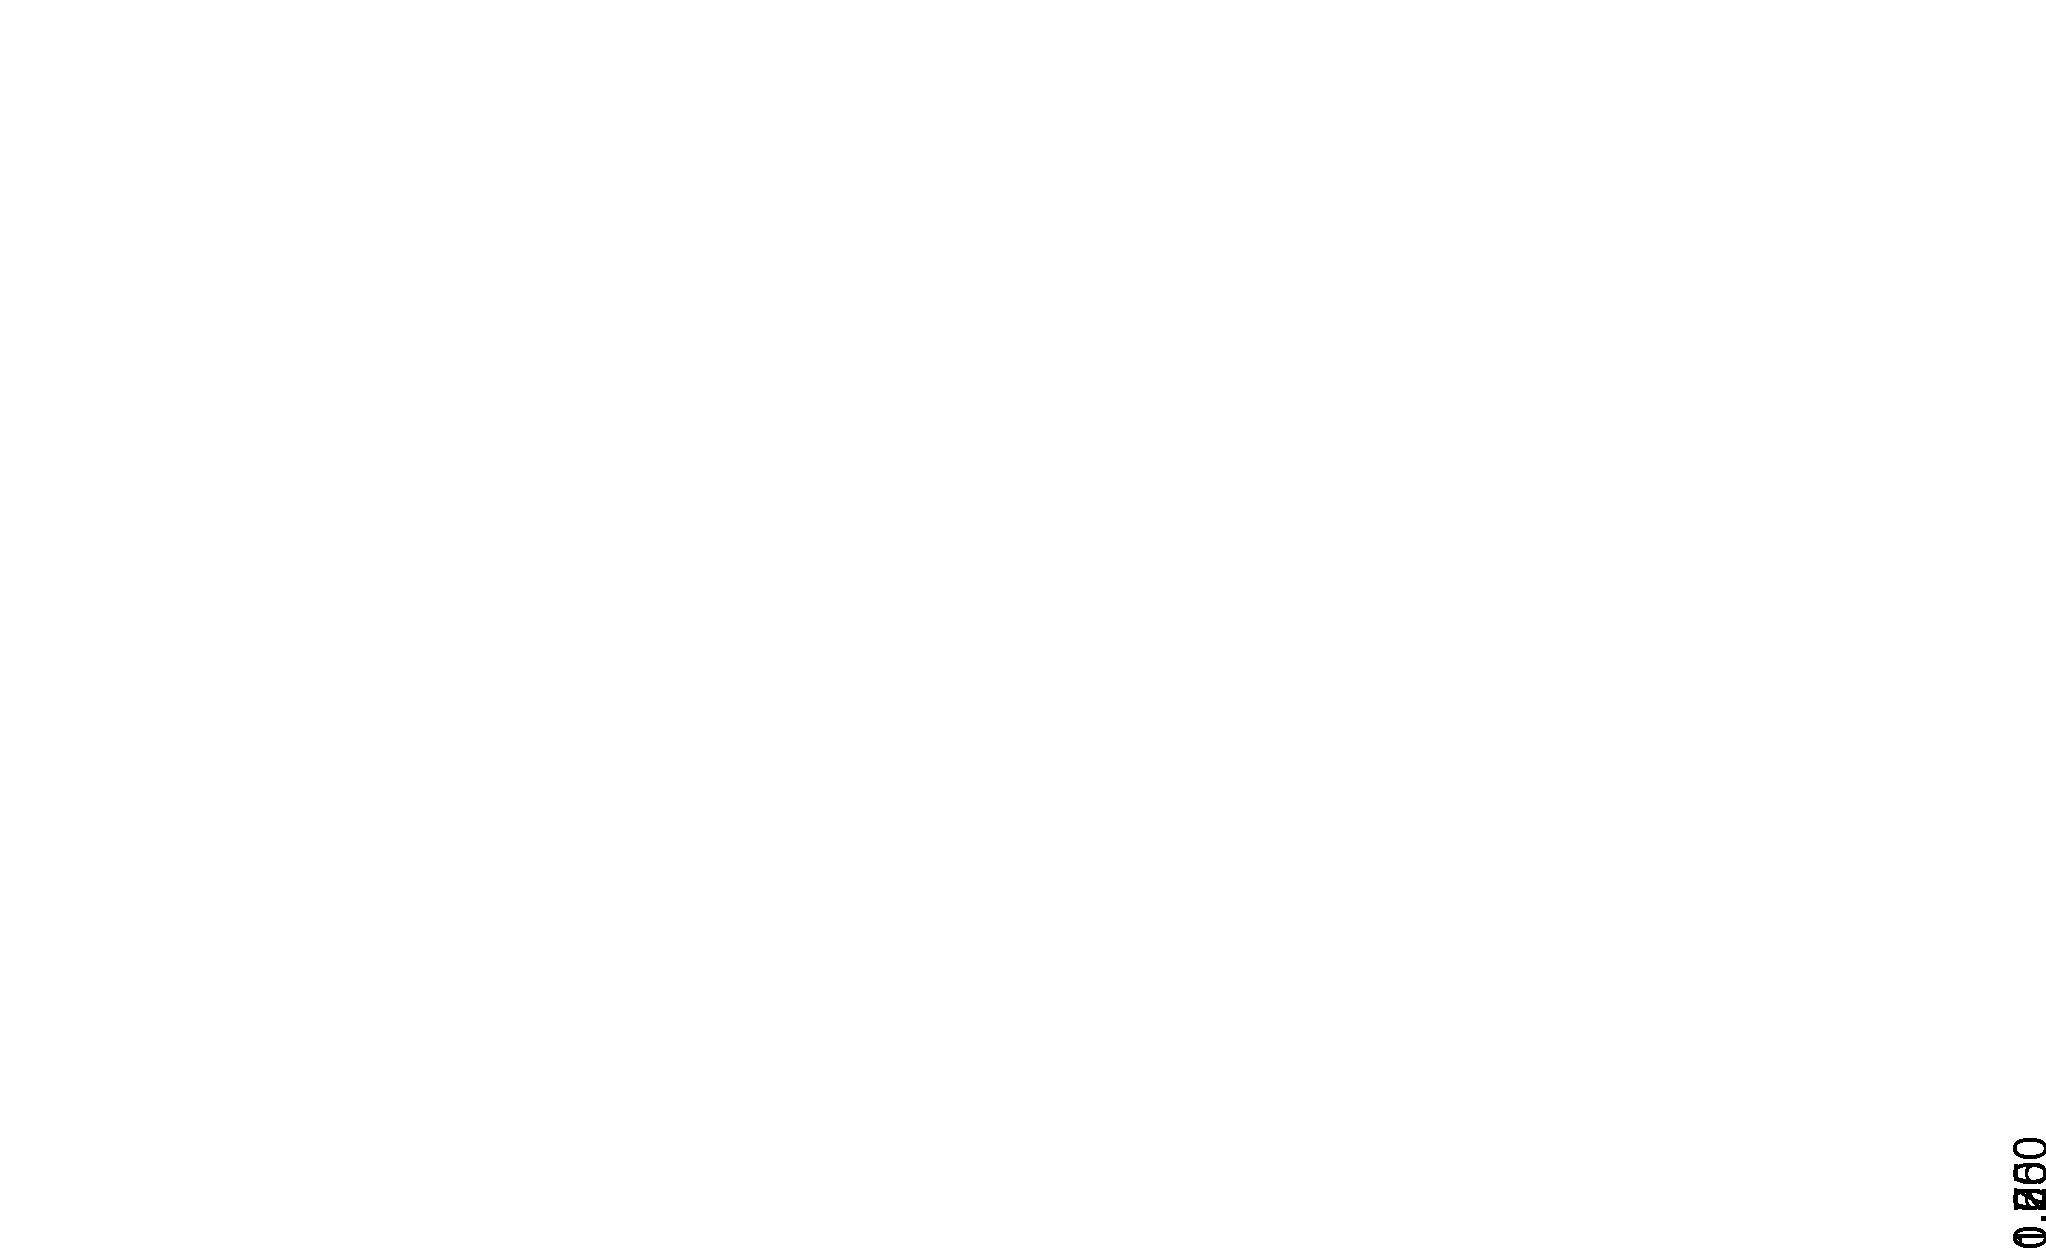
\includegraphics[scale=0.2]{mesh}
	\end{center}
	\vspace{-20pt}
	\caption{Coarse version of the mesh}
	\vspace{-10pt}
\end{wrapfigure}
The model consists of a spinal cord surrounded by space filled with CSF. The cord has a diameter of 10 mm and the fluid space has a diameter of 18 mm. The model also has a inner central spinal canal, 2 mm in diameter. The central spinal canal has height 4 cm and is placed in the center of the mesh which has heigth 6 cm.
\\
\\
\\
\\
\\
\subsection{Governing equations}
\subsection*{Fluid Space}
The fluid in the SAS as well as the central spinal canal is governed by the Navier-Stokes equations
\begin{align}
	\pdi{u_f}{t} + u\cdot \nabla u = -\frac{1}{\rho_f}\nabla p_f + \frac{1}{\rho} \nabla \cdot 		\tau + F&& \text{ in } \Omega_f 
	\\
	\pdi{\rho}{t} +\nabla \cdot(\rho u_f) = 0 && \text{ in } \Omega_f
\end{align}

where $u_f$ is the fluid velocity, $\rho_f$ is the fluid denisty, $\tau$ is the stress tensor and $F$ are all external volume forces. In addition to the equations (1)-(2) comes boundary conditions at the domain boundary. When solving the euqations numerically, manipulation of the coupled equations into simpler equations may lead to problems involving the boundary conditions. Therefore a proper choice of boundary conditions is crucial for stability and existence. 
\\
In this case we will consider incompressible flows, where $\rho$ is constant and $\nabla \cdot u = 0$. The stress tensor is given by
\[ \tau = 2 \mu \epsilon(u_f) \]
where $\epsilon(u_f) = \frac{1}{2}(\nabla u_f + (\nabla u_f)^T)$
When taking the divergence of the stress tensor the Navier-Stokes equations for incompressible flows take the form

\begin{align}
	\pdi{u_f}{t} + u\cdot \nabla u_f = -\frac{1}{\rho}\nabla p_f + \nu \nabla ^2 u_f + F && 	\text{ in } \Omega_f 
	\\
	\nabla \cdot u_f = 0 && \text{ in } \Omega_f
\end{align}

\subsection*{Spinal Cord}
The spinal cord is modeled as a poroelastic medium, which allows for some fluid to flow from the SAS to the central spinal canal. In this case the Biot-equations have been used to include both elasticity and flow in the spinal cord.
	\begin{align} -\mu \nabla ^2 u_s - (\lambda + \mu)\nabla \nabla \cdot u_s - \nabla p_s = 0 		&& \text{ in } \Omega_s \\
	(\nabla \cdot u_s)_t - \nabla \cdot (\kappa \nabla p_s) = 0 && \text{ in } \Omega_s
\end{align}
Here, $\kappa \nabla p_s$ represents the fluid velocity in the porous medium. $p_s$ is the pressure in the fluid occupying the pores. 
\subsection{Weak form}
Equations (3) and (5) will be multiplied by a vector test function, v, and equations (4) and (6) with a scalar test function, q. The equations are then integrated over the entire domain. By using two different test functions the coupled equations can be written as one weak formulation each
\begin{align}
	\int_{\Omega_f} \pdi{u_f}{t}\cdot v \mathrm{d}x &+ \int_{\Omega_f}(u_f \cdot \nabla u_f)\cdot v \mathrm{d}x = \frac{1}{\rho} \int_{\Omega_f} \nabla \cdot v \, p_f \mathrm{d}x - \nu \int_{\Omega_f} \nabla u : \nabla v \mathrm{d}x \nonumber
	\\& - \frac{1}{\rho}\int_{\partial \Omega_f} p v\cdot n \, \mathrm{d}S + \nu \int_{\partial \Omega_f} \nabla u \cdot v \cdot n \,\mathrm{d}S + \int_{\Omega_f} \nabla \cdot u \, q\, \mathrm{d}x 
\end{align}
And for the fluid and structure movement in the cord:
\begin{align}
	\mu \int_{\Omega_s} \nabla u_s : \nabla v \mathrm{d}x
 + (\mu + \lambda) \int_{\Omega_s}\nabla \cdot u_s \nabla \cdot v \mathrm{d}x
 - \mu \int_{\partial \Omega_s}\nabla u_s \cdot v \cdot n \mathrm{d}S \nonumber \\ 
 -(\lambda + \mu) \int_{\partial \Omega_s}\nabla \cdot u v \cdot n \mathrm{d}S 
 = \frac{1}{\rho} \int_{\Omega_s} \nabla \cdot v \, p_s \mathrm{d}x 
 - \frac{1}{\rho}\int_{\partial \Omega_f} p v\cdot n \, \mathrm{d}S  \nonumber \\
 + \nu \int_{\partial \Omega_s} \nabla u \cdot v \cdot n \,\mathrm{d}S
 + \int_{\Omega_s} \pdi{(\nabla \cdot u_s)}{t} q \mathrm{d}x 
 + \int_{\Omega_s} k \nabla p_f \cdot \nabla q \mathrm{d}x 
 - \int_{\partial \Omega_s} q \kappa \nabla p_f \cdot n \mathrm{d}S
\end{align}
